% Figure from MATH 556 notes, section 20. Compile with the notes preamble.
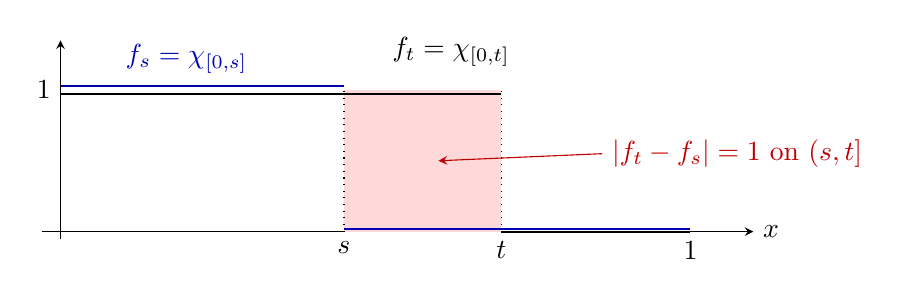
\begin{tikzpicture}[x=8cm, y=1.8cm, >=stealth]
    \draw[->] (-0.03,0) -- (1.1,0) node[right] {$x$};
    \draw[->] (0,-0.05) -- (0,1.35);
    \node[left] at (0,1) {$1$};
    \fill[red!15] (0.45,0) rectangle (0.7,1);
    \draw[thick, blue!70!black] (0,1.03) -- (0.45,1.03);
    \draw[thick, blue!70!black] (0.45,0.02) -- (1,0.02);
    \draw[thick] (0,0.97) -- (0.7,0.97);
    \draw[thick] (0.7,0) -- (1,0);
    \draw[dotted] (0.45,0) -- (0.45,1); \draw[dotted] (0.7,0) -- (0.7,1);
    \node[below] at (0.45,0) {$s$}; \node[below] at (0.7,0) {$t$}; \node[below] at (1,0) {$1$};
    \node[blue!70!black, anchor=south] at (0.2,1.05) {$f_s = \chi_{[0,s]}$};
    \node[anchor=south] at (0.62,1.1) {$f_t = \chi_{[0,t]}$};
    \draw[->, red!75!black] (0.86,0.55) -- (0.6,0.5);
    \node[red!75!black, anchor=west] at (0.86,0.55) {$|f_t - f_s| = 1$ on $(s,t]$};
\end{tikzpicture}
